% Target: IEEE Transactions on Instrumentation and Measurement (Q1). IEEEtran journal mode.
\documentclass[journal]{IEEEtran}

\usepackage{amsmath,amssymb}
\usepackage{graphicx}
\usepackage{booktabs}
\usepackage{multirow}
\usepackage{siunitx}
\usepackage{xcolor}
\usepackage{cite}
\usepackage[hidelinks]{hyperref}
\usepackage{tikz}
\usetikzlibrary{positioning,arrows.meta,fit}

\sisetup{detect-all}
\newcommand{\best}[1]{\textbf{#1}}
% Remove before submission: highlights statements the authors still have to confirm.
\newcommand{\todo}[1]{\textcolor{red}{[TODO: #1]}}

\begin{document}

\title{Physics Helps When Data Are Scarce: Hybrid DeepONet--PINN Reconstruction of Full-Chip Thermal Maps from Sparse Sensors}

\author{Ruchika~Todi,
        Siya~Patil,
        Smriti~Prashanth~Vasisht,
        Vipul~Reddy~Gundalu,
        and~Rashmi~R%
\thanks{The authors are with the Department of Information Science and Engineering, B.M.S. College of Engineering, Bengaluru 560019, India.
Corresponding author: \todo{name and e-mail}.}}

\markboth{IEEE Transactions on Instrumentation and Measurement}%
{Todi \MakeLowercase{\textit{et al.}}: Physics Helps When Data Are Scarce}

\maketitle

\begin{abstract}
On-chip thermal sensors measure temperature at only a few points, yet thermal management needs the full map of the die.
We treat this virtual-sensing task as an operator-learning problem and study when knowledge of the governing heat equation improves a neural reconstruction, with the deep operator network (DeepONet) as the learned model throughout.
We compare a purely data-driven DeepONet, a physics-informed neural network (PINN) fitted per chip from its sensors and the steady heat equation alone, and three hybrids: physics as an extra training loss of the DeepONet, a validation-weighted blend of DeepONet and PINN, and a heat-equation correction of the DeepONet at the sensors; gappy proper orthogonal decomposition (POD) is the classical baseline.
Sensors are placed by POD-QR and corrupted by a realistic noise, offset and quantisation model.
On 700 simulated $12\times12$\,mm dies the DeepONet reaches 11.5\%, 8.6\% and 6.1\% relative $L_2$ error with 5, 8 and 10 sensors when trained on 500 chips, and physics as a loss term changes nothing measurable.
Physics as a separate estimator behaves differently: the blend is never worse than its better component, and its gain grows as training data shrink, from at most 0.4 percentage points with 500 training chips to 2.9--3.9 points (about one third of the error) with 25.
The same holds on measured infrared maps of two Intel CPUs: when the DeepONet sees only 2 or 4 of 13 training workloads, the physics-corrected hybrid roughly halves its error at 8 and 10 sensors (for example 0.36 to 0.16 relative to the temperature rise) and beats the per-frame PINN at 8 sensors, while with all workloads the gain is small and gappy POD is competitive.
We explain the failure of physics as a loss by a 33\% residual of the reference maps in the discretised heat equation, and conclude that physics is most valuable as an independent estimator combined with a learned operator when training data are scarce.
\end{abstract}

\begin{IEEEkeywords}
Thermal map reconstruction, virtual sensing, deep operator network (DeepONet), physics-informed neural networks, hybrid models, data efficiency, sparse sensor placement.
\end{IEEEkeywords}

%=====================================================================
\section{Introduction}
\IEEEPARstart{P}{ower} density in modern processors keeps rising, and with it the cost of local hot spots: they shorten device lifetime, force frequency throttling, and must be found both during design validation and in the field \cite{skadron2003temperature,brooks2001dtm}.
Processors therefore carry digital thermal sensors (DTS), but area, power and routing limit them to a few per die, so the hottest point is usually not where a sensor sits.
Infrared (IR) imaging gives the full map but needs an open package and an external camera, and numerical solvers need the power map, which is not observed at run time.
Reconstructing the full thermal map from a few sensor readings, a virtual-sensing problem, is therefore a measurement task of practical importance \cite{nowroz2010thermal,ranieri2012eigenmaps,sadiqbatcha2022tracking}.

From a neural-network point of view the task is operator learning: a network must map a small, noisy set of point measurements to a whole field.
Data-driven neural operators such as the deep operator network (DeepONet) \cite{lu2021deeponet} learn this map from many examples and then reconstruct a new chip in one forward pass, but their accuracy depends on how many training maps exist, and for a new chip design or a new measurement campaign there may be very few.
Physics-informed neural networks (PINNs) \cite{raissi2019pinn,karniadakis2021piml,cuomo2022sciml} need no training set: they fit a network to one chip's readings while penalising the residual of the governing partial differential equation (PDE), at the cost of an optimisation per chip.
The literature argues that physics improves accuracy and data efficiency \cite{karniadakis2021piml,willard2022integrating,cai2021heat,du2025review}.
Two questions remain open for this application: \emph{when}, in terms of training-set size, does physics help a learned reconstruction, and \emph{how} should it be added, as an extra loss term \cite{wang2021pideeponet} or as a separate estimator combined with the network?

We answer both with controlled experiments in which the DeepONet is the learned model throughout, every model shares the same data splits, sensor layout, noise model and metrics, and the training-set size is varied deliberately.
Our research questions are:
\begin{itemize}
\item \textbf{RQ1:} How accurately can a DeepONet reconstruct a full-chip thermal map from 5 to 10 noisy sensors, compared with a pure PINN and the classical gappy POD?
\item \textbf{RQ2:} Does physics help, in which form, and how does its benefit depend on the number of training samples?
\item \textbf{RQ3:} Do the conclusions hold on measured IR maps of commercial processors?
\end{itemize}

Our contributions are:
\begin{enumerate}
\item A controlled comparison of a pure-ML DeepONet, a pure per-chip PINN, and three DeepONet--physics hybrids (physics loss, validation-weighted blend, physics correction) against gappy POD, on 700 simulated dies with POD-QR sensor placement and a realistic sensor model.
\item A data-scarcity study on simulated (25 to 500 chips) and measured (2 to 13 workloads) data, with paired bootstrap confidence intervals, showing that physics as a separate estimator gives little with plentiful data but cuts the error by one third to one half when training data are scarce, while physics as a loss term gives no measurable gain at any size.
\item An interpretation of the hybrid as a bias--variance trade-off, confirmed by the validation-selected blend weights, and a diagnosis of why a PDE loss fails here: the reference maps leave a 33\% residual in the discretised heat equation.
\item A justification of the measurement design (POD-QR placement, noise model, metrics) for thermal management, and a summary of the alternative architectures we explored and why the DeepONet was retained.
\end{enumerate}

Section~\ref{sec:related} reviews related work, Section~\ref{sec:problem} states the problem, Section~\ref{sec:data} describes data, sensors and metrics, Section~\ref{sec:methods} the models, Sections~\ref{sec:sim} and~\ref{sec:real} report results, Section~\ref{sec:discussion} discusses them, Section~\ref{sec:other} summarises other architectures explored, and Section~\ref{sec:conclusion} concludes.

%=====================================================================
\section{Related Work}\label{sec:related}

\subsection{Full-chip thermal map estimation}
Early work recovered full maps from a few sensors with linear models built from simulated or measured maps, using spectral or eigen-decompositions and placing sensors to make the inverse well conditioned \cite{nowroz2010thermal,ranieri2012eigenmaps}.
Gappy POD \cite{everson1995gappy,willcox2006gappy} and POD-QR placement \cite{manohar2018sensor} are the general form of this idea and remain strong baselines.
Learning-based estimators followed: a generative adversarial network trained on IR images of a commercial CPU \cite{jin2020gan}, models that track temperature from performance counters \cite{sadiqbatcha2022tracking}, and a public IR dataset of commercial CPUs, GPUs and TPUs \cite{lu2024dataset}, which we use.
Physics-enforced networks have been used for full-chip thermal analysis when the power map is known \cite{chen2023parametric} and for microprocessor--heat-sink modelling \cite{son2023microprocessor}.
In our setting the power map is unknown and only sparse, noisy readings are available.

\subsection{Operator learning and physics-informed networks}
DeepONet \cite{lu2021deeponet} approximates an operator with a branch network that encodes the input function from its values at fixed points and a trunk network that encodes the output coordinate, backed by a universal approximation theorem for operators.
The Fourier neural operator (FNO) \cite{li2021fno} learns the operator in spectral space on a grid.
Both have physics-informed variants that add the PDE residual to the training loss \cite{wang2021pideeponet,li2024pino}.
PINNs \cite{raissi2019pinn} minimise a data misfit plus the PDE residual computed by automatic differentiation and have been used for forward and inverse heat-transfer problems with sparse measurements \cite{cai2021heat}; they are known to be hard to optimise when loss terms compete \cite{wang2021gradient,krishnapriyan2021failure}.
Most studies add physics to the loss; few compare this with combining an independent physics estimate with a learned one, and fewer vary the amount of training data systematically, which is the focus here.

%=====================================================================
\section{Problem Formulation}\label{sec:problem}

Let $T(\mathbf{x})$ be the steady temperature on the die $\Omega=[0,L]^2$, sampled on an $H\times W$ grid.
$N$ sensors at fixed positions $\{\mathbf{x}_i\}_{i=1}^N$ return noisy, quantised readings $y_i$; the ambient temperature $T_\mathrm{amb}$ is known for the simulated dies.
The block layout and power map are not available.
We seek an estimator $\hat T=\mathcal G(\{\mathbf{x}_i,y_i\},T_\mathrm{amb})$ of the full field.
A learned estimator $\mathcal G_\phi$ is trained on $n$ example maps by minimising the empirical risk; its generalisation error grows as $n$ shrinks, which is the regime where prior knowledge should matter most.

For the simulated dies the temperature satisfies the compact two-dimensional HotSpot model \cite{huang2006hotspot}
\begin{equation}\label{eq:pde}
-\nabla\cdot\big(t_\mathrm{die}\,k(T)\,\nabla T\big) + h_\mathrm{eff}\,(T-T_\mathrm{amb}) = q(\mathbf{x},T),
\end{equation}
with adiabatic lateral edges ($\partial T/\partial n=0$), die thickness $t_\mathrm{die}$, an effective vertical conductance $h_\mathrm{eff}$ to the heat sink, a temperature-dependent silicon conductivity $k(T)$ \cite{glassbrenner1964silicon}, and a power density $q$ of block-wise dynamic power plus leakage growing as $\exp(\beta(T-25\,^\circ\mathrm{C}))$.
With $\theta=(T-T_\mathrm{amb})/S$ for a temperature scale $S$ and coordinates scaled to the unit square,
\begin{equation}\label{eq:nondim}
-\varepsilon\,\nabla\cdot\big(k(T)\nabla\theta\big) + \theta = \tilde q, \qquad \varepsilon=\frac{t_\mathrm{die}}{h_\mathrm{eff}L^2}\approx 5.6\times10^{-4},
\end{equation}
a screened Poisson equation.
The small $\varepsilon$ means heat spreads only a short distance laterally ($\sqrt\varepsilon L\approx0.3$\,mm) before it leaves vertically, so a hot block far from every sensor leaves almost no trace in the readings.
This makes the inverse problem ill-posed at low sensor counts, whatever the estimator.

%=====================================================================
\section{Data, Sensors and Metrics}\label{sec:data}

\subsection{Simulated dies}
Simulation gives exact ground truth, full control over the floorplans and enough samples to vary the training-set size.
We generated 700 dies of $12\times12$\,mm with a HotSpot-style solver \cite{huang2006hotspot}.
Each die holds up to 8 non-overlapping rectangular blocks (2 to 8 drawn; blocks that cannot be placed are skipped) of four types, CPU, GPU, cache and memory controller, with dynamic power densities drawn from type-specific ranges between 5 and 150\,W/cm$^2$, uniform within a block, and leakage fractions of 3--5\% with $\beta=0.012$\,K$^{-1}$.
Ambient temperature is uniform in $[25,45]\,^\circ$C, $t_\mathrm{die}=500\,\mu$m and $h_\mathrm{eff}=6256$\,W/(m$^2$K).
Equation~(\ref{eq:pde}) is solved by Picard iteration (inner loop for $k(T)$, outer loop for leakage) on a $512\times512$ mesh, and every fourth node is kept, giving $128\times128$ maps.
Generating the reference on a finer mesh than any model uses avoids an ``inverse crime'' \cite{wirgin2004inverse}, in which a method is tested on data produced by its own discretisation and looks better than it would on real data.
The dies are split 500/100/100 into training, validation and test sets; floorplans are never shared between splits.
\todo{Confirm $t_\mathrm{die}$, $h_\mathrm{eff}$ and the power ranges; PROTOCOL.md marks them as assumptions not yet traced to a source.}

\subsection{Measured IR maps}
To test transfer to real hardware we use the public dataset of Lu and Tan \cite{lu2024dataset}, which records IR maps of commercial processors running benchmark workloads.
We keep the two Intel CPUs, i5-3337U ($177\times166$ pixels, 5 workloads) and i7-8650U ($185\times154$ pixels, 19 workloads), with 100 consecutive frames per workload.
The Ryzen 7 4800U and RTX 4060 recordings were excluded because their maps contain a fixed pattern (printed text, a grid structure) that does not change with the thermal state, an emissivity artefact rather than temperature.
Consecutive frames are nearly identical, so splits are made by whole workload to prevent leakage: i5 3/1/1 workloads (300/100/100 frames) and i7 13/3/3 workloads (1300/300/300 frames) for training, validation and test.
Power maps, die stack and ambient temperature are unknown for these parts.

\subsection{Sensor placement by POD-QR}
Sensors are placed by POD-QR \cite{manohar2018sensor}.
The training maps (normalised per sample for the simulated set) are centred and decomposed by singular value decomposition; the leading $r$ POD modes holding 95\% of the energy are kept ($r=11$ for the simulated set), giving a basis $\Psi_r$.
QR factorisation with column pivoting of $\Psi_r^\top$ ranks the grid points, and the first 5, 8 and 10 pivots, excluding a 3-cell border, form nested layouts ($5\subset8\subset10$).
Layouts are fitted on training data only and fixed for all chips.

We chose POD-QR for four reasons.
(i) It targets reconstruction directly: column pivoting greedily maximises the volume (determinant) of the sampled mode matrix $\Psi_r(\mathbf{x}_\mathcal{S},:)$, which bounds how much sensor noise is amplified when the field is recovered from the readings; the same selection underlies the discrete empirical interpolation method and its QR variant, which have a priori error bounds \cite{chaturantabut2010deim,drmac2016qdeim}.
(ii) It has been shown to outperform random and uniform placements for reconstructing fields with low-dimensional structure \cite{manohar2018sensor}, and thermal maps of processors are such fields; eigen-decomposition-based placement was found effective specifically for multicore thermal maps \cite{ranieri2012eigenmaps,nowroz2010thermal}.
(iii) It is cheap (one SVD and one pivoted QR) and deterministic, so all models see the same layout.
(iv) Its layouts are nested, so the 5- and 8-sensor results are subsets of the 10-sensor design, as when a designer adds sensors.
Because POD-QR is also the natural partner of gappy POD, it gives the classical baseline its best conditions; any advantage of the networks is therefore not due to a layout that suits them.
We did not compare alternative placements; this is a limitation (Section~\ref{sec:discussion}).

\subsection{Sensor model}
Each reading is the true temperature plus a per-sensor calibration offset $\sim\mathcal N(0,0.5^2)\,^\circ$C and Gaussian noise $\sigma=1\,^\circ$C, rounded to 1\,$^\circ$C, a model of a typical DTS.
Readings are generated once with fixed seeds and stored, so every model receives identical inputs; the true values are used only for scoring.
The same model is applied to the IR maps, where a sensor is one image pixel.

\subsection{Evaluation metrics and why they fit the application}
Table~\ref{tab:metrics} lists the metrics; all are computed on non-sensor nodes only, so a model gains nothing from reproducing the values it was given.

\begin{table}[t]
\caption{Metrics, computed on non-sensor nodes, and what each captures for thermal management.}
\label{tab:metrics}
\centering
\footnotesize
\setlength{\tabcolsep}{3pt}
\begin{tabular}{@{}p{0.27\columnwidth}p{0.66\columnwidth}@{}}
\toprule
Metric & Role \\
\midrule
Relative $L_2$ & $\|\hat T-T\|_2/\|T\|_2$. Scale-free whole-map accuracy; the standard measure in operator learning \cite{lu2021deeponet,li2021fno}, so results are comparable with that literature. \\
MAE, RMSE ($^\circ$C) & Typical and large-error-weighted deviation in physical units, read directly against a thermal margin. \\
Peak error ($^\circ$C) & $\max\hat T-\max T$. Throttling and protection act on the maximum temperature \cite{skadron2003temperature,brooks2001dtm}; under-prediction (negative) is the dangerous direction. \\
Hotspot error (cells) & Distance between predicted and true maxima. Decides which unit is throttled or cooled. \\
Rise error (real maps) & $\|\hat T-T\|_2/\|T-\min T\|_2$. Normalises by the spatial variation rather than the absolute level. \\
\bottomrule
\end{tabular}
\end{table}

No single number captures fitness for thermal management, which needs the right map, the right peak and the right location, so we report all five.
Relative $L_2$ is the headline because it is scale-free and standard, but on its own it can mislead: real maps sit at 35--95\,$^\circ$C with only a few degrees of variation, so a model that predicts the average training map already scores about 8--17\% relative $L_2$ while carrying no information about the chip.
For the real maps we therefore use the rise error, under which the training-mean map scores about 0.9 and differences between models become visible.
MAE and RMSE add physical units; their gap indicates whether error is spread out or concentrated at hot spots.
Peak and hotspot errors capture what a controller acts on; they are single-point statistics and can jump when two regions are almost equally hot, so we read them as averages over the 100 test chips and not per chip.
Inference time is reported because a run-time monitor must update the map within a control interval.

%=====================================================================
\section{Methods}\label{sec:methods}

\subsection{Choice of DeepONet as the learned model}
We use DeepONet as the learned model for three reasons.
Its branch network takes the sensor positions and readings directly, so scattered measurements need no interpolation onto a grid, and its trunk network can be queried at any coordinate, so one model serves the $128\times128$ simulated maps and the non-square IR maps alike.
It reconstructs a map in tens of milliseconds, fast enough for run-time use.
And it had the lowest error among the architectures we tried under the same protocol (Section~\ref{sec:other}), with a structure to which physics can be added without changing the network, so that comparisons isolate the effect of physics.
All networks use PyTorch and Adam \cite{kingma2015adam} with cosine learning-rate decay, keep the checkpoint with the lowest validation error, and are scored once on the test set.

\begin{figure}[t]
\centering
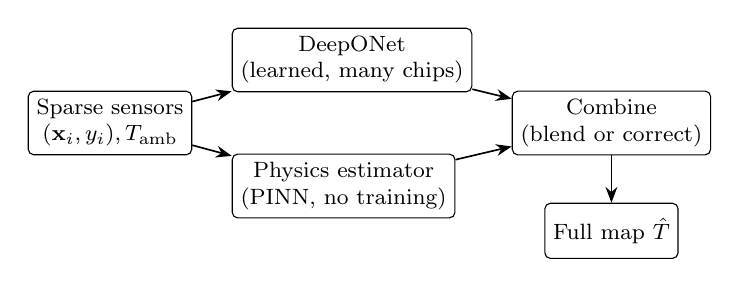
\begin{tikzpicture}[
  box/.style={draw, rounded corners=2pt, align=center, font=\footnotesize, minimum height=7mm, inner sep=3pt},
  arr/.style={-{Stealth[length=2mm]}, semithick}]
\node[box] (s) {Sparse sensors\\$(\mathbf{x}_i, y_i), T_\mathrm{amb}$};
\node[box, right=5mm of s, yshift=8mm] (d) {DeepONet\\(learned, many chips)};
\node[box, right=5mm of s, yshift=-8mm] (p) {Physics estimator\\(PINN, no training)};
\node[box, right=5mm of d, yshift=-8mm] (b) {Combine\\(blend or correct)};
\node[box, below=6mm of b] (m) {Full map $\hat T$};
\draw[arr] (s) -- (d); \draw[arr] (s) -- (p);
\draw[arr] (d) -- (b); \draw[arr] (p) -- (b); \draw[arr] (b) -- (m);
\end{tikzpicture}
\caption{Hybrid reconstruction with physics as a separate estimator. The DeepONet, learned from many chips, and a physics estimator fitted to one chip's sensors each predict the map; they are combined with settings chosen on validation data. The alternative, physics as a loss term, adds the heat-equation residual to the DeepONet's training loss instead.}
\label{fig:overview}
\end{figure}

\subsection{Pure ML: DeepONet}
The DeepONet \cite{lu2021deeponet} predicts
\begin{equation}
\hat\theta(\mathbf{x}) = \mathbf{b}(\mathbf{s})^\top\mathbf{t}(\mathbf{x}) + b_0,
\end{equation}
where the branch network $\mathbf{b}$ receives $\mathbf{s}=[x_1,y_1,\theta_1,\dots,x_N,y_N,\theta_N]$ (positions and scaled readings) and the trunk network $\mathbf{t}$ a query coordinate in $[0,1]^2$.
Both are tanh multilayer perceptrons of width 128 (3 branch and 4 trunk hidden layers) with $p=128$ outputs, giving 118,017, 119,169 and 119,937 parameters for 5, 8 and 10 sensors.
The trunk learns a set of $p$ spatial basis functions shared by all chips and the branch learns, for each chip, their coefficients from the readings, so the model is a learned, nonlinear generalisation of a POD expansion.
Temperatures are scaled as $\theta=(T-T_\mathrm{amb})/S$ with one global $S$, the largest rise in the training set.
Training minimises the mean squared error at 1024 random grid points per chip, with batches of 32 chips, learning rate $10^{-3}$ decaying to $10^{-5}$, up to 400 epochs and early stopping on validation error (checked every 10 epochs, patience 10).
One network is trained per sensor count for 5 seeds (about 2 minutes each on a CPU).
For reduced training sets the number of epochs is raised so that the number of optimisation steps matches the full-data runs.
On the real maps the same network is trained for 6000 steps.

\subsection{Pure PINN: per-chip physics-only network}
The PINN uses no training set.
For each test chip a tanh network of 4 layers by 64 units represents $\theta(\mathbf{x})$; it receives $(\cos\pi x,\cos\pi y)$ instead of $(x,y)$, which makes $\partial\theta/\partial n=0$ on every edge for any weights, so the adiabatic boundary condition holds exactly.
The unknown dynamic power is learned as a sum of 6 Gaussian blobs with trainable amplitudes, centres and widths, with leakage applied as $1+f\exp(\beta(T-25))$, $f=0.0425$.
The loss is
\begin{equation}
\mathcal L = \frac{1}{M}\sum_{j=1}^{M} R(\mathbf{x}_j)^2 + \lambda_\mathrm{d}\frac{1}{N}\sum_{i=1}^{N}\big(\hat\theta(\mathbf{x}_i)-\theta_i\big)^2,
\end{equation}
with $R$ the residual of (\ref{eq:nondim}) computed by automatic differentiation at $M=2048$ random collocation points and $\lambda_\mathrm{d}=100$.
Optimisation runs 5000 Adam steps and 2000 L-BFGS steps, about 3 minutes per chip on a 4-core CPU, one seed.
On the IR maps the same code is applied per frame with the die mapped to the unit square, $t_\mathrm{die}$ and $h_\mathrm{eff}$ chosen so that $\varepsilon$ matches its simulated value, leakage off, the sink temperature set to the minimum of the training maps, and a shortened budget of 600 Adam and 100 L-BFGS steps (about 2 minutes per frame).

\subsection{Hybrid 1: physics as a loss (physics-informed DeepONet)}
The DeepONet gains a second output, a non-negative dynamic power density $\hat q$, computed from the same branch embedding; the temperature trunk receives $(\cos\pi x,\cos\pi y)$ for exact adiabatic edges.
The residual of (\ref{eq:nondim}) linking $\hat\theta$ and $\hat q$ is evaluated at 64 collocation points per chip and added to the data loss with weight 0.1, ramped up from zero over the first 40 epochs \cite{wang2021pideeponet}.
$\hat q$ is never supervised, so the physics term needs no extra data.
An optional second stage refines each test chip with the physics loss.

\subsection{Hybrid 2: physics as a separate estimator (blend)}
The blend combines the two independent estimators,
\begin{equation}\label{eq:blend}
\hat T_\mathrm{blend} = w\,\hat T_\mathrm{DeepONet} + (1-w)\,\hat T_\mathrm{PINN},
\end{equation}
with $w\in\{0,0.1,\dots,1\}$ chosen per sensor count and training-set size by the mean relative $L_2$ error on the 100 validation chips, then fixed and applied once to the test chips.
Because $w=0$ and $w=1$ are allowed, the blend can fall back on either component.
It uses the seed-0 DeepONet.

\subsection{Hybrid 3: physics correction (real maps)}
For the IR maps the power map and material constants are unknown, so the physics enters through a linearised form of (\ref{eq:pde}), $(1-\ell^2\nabla^2)(T-T_0)=q/h$, with adiabatic edges and a decay length $\ell$ in pixels.
The unknown source is expanded in Gaussian bumps on a coarse grid; the response of each bump is computed with a discrete cosine transform, which enforces the adiabatic edges.
Fitting the bump amplitudes and $T_0$ to the readings by ridge regression gives a physics-only reconstruction that uses no training maps.
The \emph{correction} hybrid fits the same response to the DeepONet's residual at the sensors, $y_i-\hat T_\mathrm{D}(\mathbf{x}_i)$, and adds it to the DeepONet map, so the learned map is pulled through the readings in a way the heat equation allows.
We also test blends of the DeepONet with the physics reconstruction and with the per-frame PINN, and a blend followed by correction.
All settings ($\ell$, bump spacing, ridge weight, blend weight) are chosen on validation frames, and the hybrid variant is fixed by one rule, the lowest mean validation error over all settings; the correction was chosen in every experiment and is reported as ``the hybrid''.

\subsection{Baselines}
\emph{Gappy POD} \cite{everson1995gappy,willcox2006gappy} fits the readings with the leading $k$ POD modes of the training maps by least squares, with $k\le N$ chosen on validation data.
It is the classical linear counterpart of the DeepONet: a fixed linear basis with coefficients from the readings.
The \emph{training-mean map} ignores the sensors and is the error of a model that learns nothing.

\subsection{Why combining helps: a bias--variance view}\label{sec:biasvar}
Write the errors of the two estimators on a chip as $e_\mathrm{D}=\hat T_\mathrm{D}-T$ and $e_\mathrm{P}=\hat T_\mathrm{P}-T$, with mean squared values $a=\mathbb E\|e_\mathrm{D}\|^2$, $b=\mathbb E\|e_\mathrm{P}\|^2$ and cross term $c=\mathbb E\langle e_\mathrm{D},e_\mathrm{P}\rangle$.
The blend error is $w^2a+(1-w)^2b+2w(1-w)c$, minimised at
\begin{equation}\label{eq:wopt}
w^\ast=\frac{b-c}{a+b-2c},
\end{equation}
where it is below $\min(a,b)$ whenever the errors are not perfectly correlated.
The two estimators sit at opposite ends of a bias--variance trade-off.
The DeepONet has low bias but its estimation error grows as the number $n$ of training maps falls, so $a=a(n)$ increases as data shrink.
The PINN has no estimation error from data, since it uses none, but it is biased by its smooth source model and by the mismatch between (\ref{eq:nondim}) and the reference maps, so $b$ does not depend on $n$.
Equation~(\ref{eq:wopt}) therefore predicts that as $n$ falls the optimal weight moves towards the physics estimator and the gain of the blend over the DeepONet grows.
Physics as a loss term, in contrast, acts as a regulariser inside one network: it can reduce variance only to the extent that the PDE agrees with the data, and it cannot supply an independent estimate.
Sections~\ref{sec:sim} and~\ref{sec:real} test these predictions.

%=====================================================================
\section{Results on Simulated Data}\label{sec:sim}

\subsection{Accuracy with 500 training chips (RQ1)}
Table~\ref{tab:sim_main} lists test errors on the 100 test chips; the number of seeds is given for every row, and multi-seed rows show mean $\pm$ standard deviation.
The DeepONet reaches 11.5\%, 8.6\% and 6.1\% relative $L_2$ error at 5, 8 and 10 sensors (MAE 4.7, 3.4 and 2.4\,$^\circ$C) and reconstructs one $128\times128$ map in 40--50\,ms on a CPU, about $4000\times$ faster than a PINN solve.
Error falls steeply with sensor count, as expected from the short heat-spreading length in (\ref{eq:nondim}).
Fig.~\ref{fig:sim_maps} shows typical reconstructions: the DeepONet finds the main hot block, but blocks between sensors are smoothed or missed, which produces the largest errors.

\begin{table*}[t]
\caption{Simulated test set (100 chips, 500 training chips). Relative $L_2$ error (\%) and MAE ($^\circ$C) on non-sensor nodes; lower is better.}
\label{tab:sim_main}
\centering
\footnotesize
\begin{tabular}{@{}llc ccc ccc@{}}
\toprule
& & & \multicolumn{3}{c}{Rel.\ $L_2$ (\%)} & \multicolumn{3}{c}{MAE ($^\circ$C)} \\
\cmidrule(lr){4-6}\cmidrule(l){7-9}
Type & Model & Seeds & $N{=}5$ & $N{=}8$ & $N{=}10$ & 5 & 8 & 10 \\
\midrule
Pure ML & DeepONet & 5 & \best{11.46}{\scriptsize$\pm$.10} & 8.62{\scriptsize$\pm$.06} & 6.13{\scriptsize$\pm$.03} & \best{4.66} & 3.37 & 2.38 \\
Pure PINN & Per-chip PINN & 1 & 13.33 & 8.80 & 6.51 & 5.19 & 3.30 & 2.39 \\
Hybrid 1 & Physics-informed DeepONet & 5 & 11.47{\scriptsize$\pm$.10} & 8.61{\scriptsize$\pm$.06} & 6.16{\scriptsize$\pm$.06} & 4.67 & 3.36 & 2.39 \\
 & \quad + per-chip physics refinement & 1 & 11.88 & 8.94 & 6.78 & 4.76 & 3.49 & 2.69 \\
Hybrid 2 & Blend (DeepONet + PINN) & 1 & 11.62 & \best{8.21} & \best{6.01} & 4.68 & \best{3.16} & \best{2.27} \\
\bottomrule
\end{tabular}
\end{table*}

\begin{figure}[t]
\centering
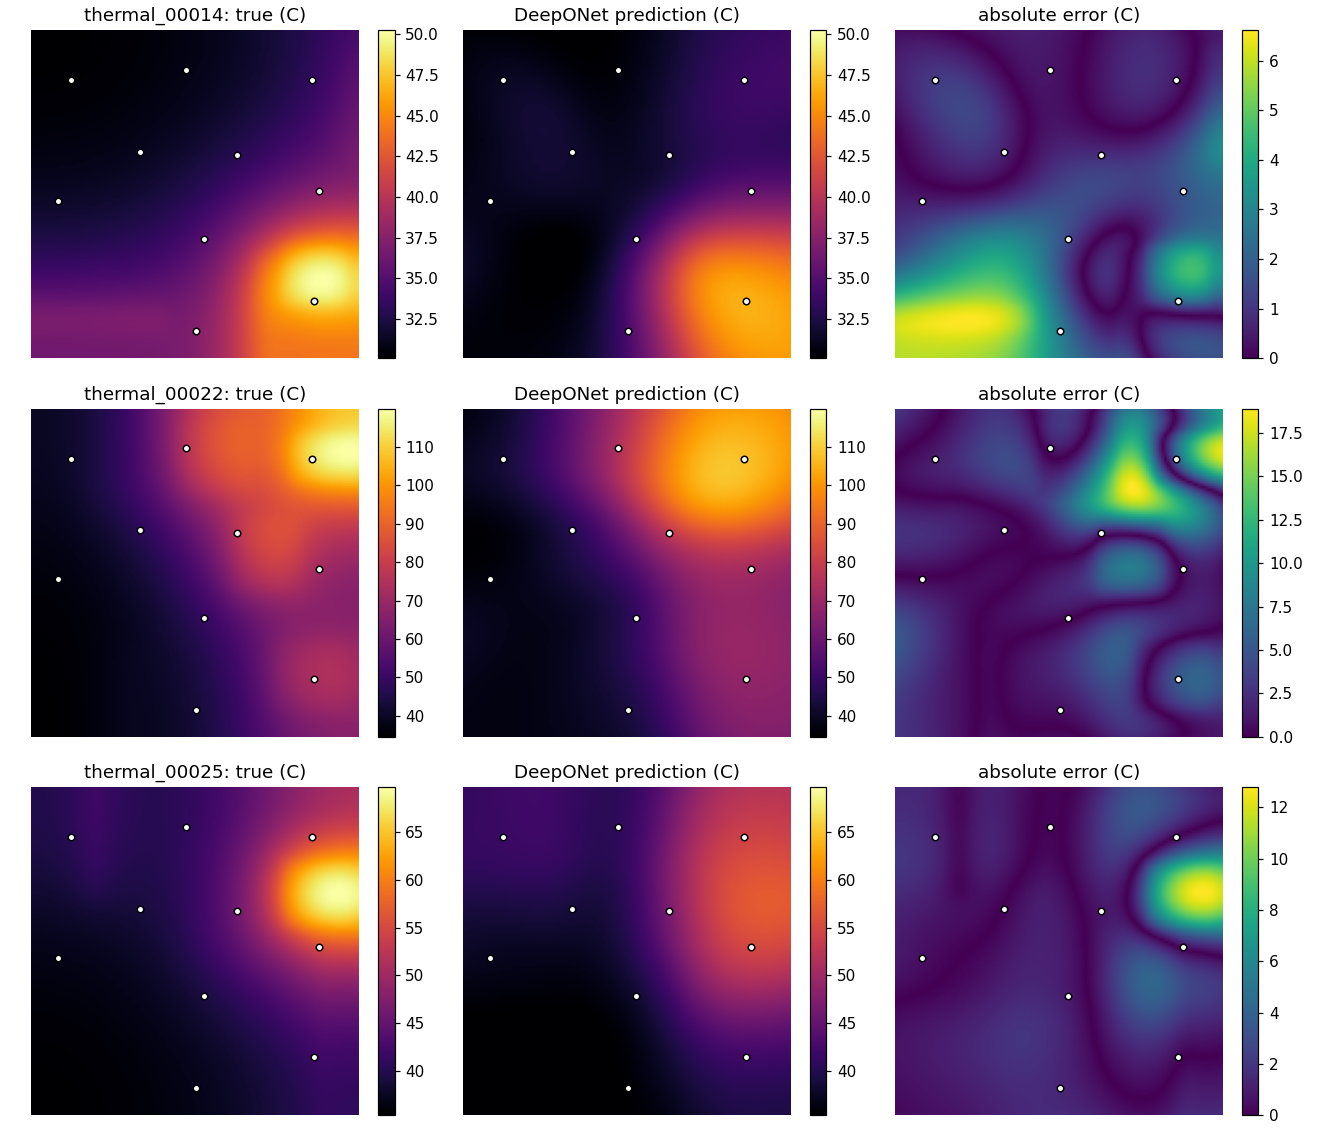
\includegraphics[width=\columnwidth]{figures/sim_maps_n10_crop.png}
\caption{DeepONet reconstructions of three simulated test chips with 10 sensors (white dots), seed 0. Left: reference; centre: prediction; right: absolute error ($^\circ$C). Errors concentrate on blocks between sensors.}
\label{fig:sim_maps}
\end{figure}

\subsection{Physics as a loss term (RQ2)}
Adding the heat-equation residual to the DeepONet's loss leaves the error unchanged within the seed spread at every sensor count (11.47 vs 11.46\%, 8.61 vs 8.62\%, 6.16 vs 6.13\%), and refining each test chip with the physics loss makes it slightly worse.
With 500 densely supervised maps the data term already pins the field, and the residual has little to add; Section~\ref{sec:discussion} explains why it can even pull the wrong way.

\subsection{Physics as a separate estimator (RQ2)}
The PINN, which sees nothing but one chip's sensors and the heat equation, is worse than the DeepONet at 5 sensors and close to it at 8 and 10.
Its errors are of a different kind (Table~\ref{tab:peak}): the DeepONet under-predicts the peak temperature by 7.4 to 13.8\,$^\circ$C, the PINN by only 2.3 to 8.0\,$^\circ$C.
A data-driven model regresses towards the average chip and flattens rare, intense hot spots, whereas the PINN's source model and the physics let it extrapolate the peak from nearby readings; its smooth sources, however, place the hotspot less precisely.
Because the errors differ, the blend gains: it has the lowest relative $L_2$, MAE and RMSE at 8 and 10 sensors (Table~\ref{tab:sim_main}).
Paired over chips (Table~\ref{tab:paired}) the blend is significantly better than the PINN at every sensor count and than the DeepONet at 8 sensors (+0.38 points, 95\% CI $[0.13,0.62]$); at 5 and 10 sensors the difference from the DeepONet is not significant with 500 training chips.

\begin{table}[t]
\caption{Peak-temperature error ($^\circ$C; negative = under-prediction) and hotspot localisation error (grid cells), 100 test chips, one seed each (DeepONet seed 0).}
\label{tab:peak}
\centering
\footnotesize
\setlength{\tabcolsep}{4pt}
\begin{tabular}{@{}l ccc ccc@{}}
\toprule
& \multicolumn{3}{c}{Peak error ($^\circ$C)} & \multicolumn{3}{c}{Hotspot error (cells)} \\
\cmidrule(lr){2-4}\cmidrule(l){5-7}
Model & $N{=}5$ & 8 & 10 & 5 & 8 & 10 \\
\midrule
DeepONet & $-13.8$ & $-9.0$ & $-7.4$ & 35.3 & \best{27.4} & \best{18.2} \\
Per-chip PINN & \best{$-8.0$} & \best{$-3.7$} & \best{$-2.3$} & 46.5 & 32.7 & 27.3 \\
Blend & $-13.3$ & $-7.2$ & $-5.5$ & \best{34.9} & 28.5 & 22.3 \\
\bottomrule
\end{tabular}
\end{table}

\begin{table}[t]
\caption{Paired comparison of the blend on the 100 test chips (500 training chips): mean reduction of relative $L_2$ error (percentage points; positive = blend better), 95\% bootstrap CI, and share of chips where the blend is better.}
\label{tab:paired}
\centering
\footnotesize
\setlength{\tabcolsep}{3.5pt}
\begin{tabular}{@{}c l c c c@{}}
\toprule
$N$ & vs & Gain (pts) & 95\% CI & Chips better \\
\midrule
\multirow{2}{*}{5} & DeepONet & $-0.03$ & $[-0.24, 0.16]$ & 63\% \\
 & PINN & $+1.71$ & $[0.82, 2.65]$ & 59\% \\
\multirow{2}{*}{8} & DeepONet & $+0.38$ & $[0.13, 0.62]$ & 67\% \\
 & PINN & $+0.59$ & $[0.22, 1.03]$ & 51\% \\
\multirow{2}{*}{10} & DeepONet & $+0.15$ & $[-0.09, 0.36]$ & 59\% \\
 & PINN & $+0.50$ & $[0.24, 0.79]$ & 69\% \\
\bottomrule
\end{tabular}
\end{table}

\subsection{Physics helps when training data are scarce (RQ2)}
We retrained the DeepONet on nested random subsets of 25, 50 and 100 training chips (5 seeds each, same number of optimisation steps) and re-selected the blend weight on validation chips; the PINN needs no training chips and is unchanged.
Fig.~\ref{fig:lowdata} and Table~\ref{tab:lowdata} show the central result of this paper.
The DeepONet degrades quickly as data shrink: from 6.1\% to 9.3\% at 10 sensors and from 8.6\% to 12.7\% at 8 sensors.
The blend does not: with 25 training chips it lowers the error to 8.8\% at 8 sensors and 6.4\% at 10 sensors, gains of 3.9 and 2.9 points (31\% of the DeepONet's error in both cases), with 95\% confidence intervals well clear of zero.
The gain shrinks steadily as data grow, to 0.4 and 0.15 points with 500 chips.

The validation-selected weight behaves as (\ref{eq:wopt}) predicts.
With 25 training chips the DeepONet receives only $w=0.1$ (8 and 10 sensors) or 0.3 (5 sensors); with 500 chips it receives 0.5 to 0.8.
As the DeepONet's estimation error grows, the data themselves move the trust to the physics estimator.
The blend is never worse than its better component by more than 0.2 points in the 12 settings and better than both in 11 of them.
Two qualifications apply.
At 25 and 50 chips much of the gain comes from the PINN itself (8.80 vs 8.78\% at 8 sensors with 25 chips); the value of the blend is that it finds the right mix automatically in every regime without knowing in advance which component is better.
At 5 sensors all methods lie between 11.5 and 13.8\%: five readings carry too little information about blocks far from them, whatever the model.

\begin{figure*}[t]
\centering
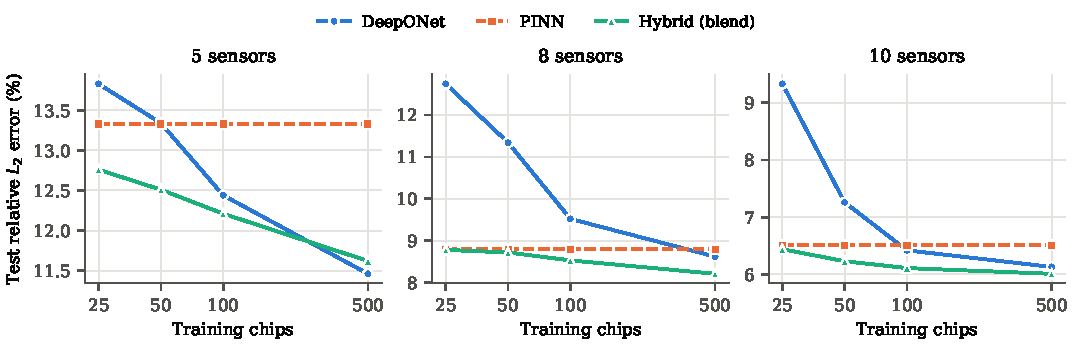
\includegraphics[width=\textwidth]{figures/low_data.pdf}
\caption{Simulated dies: test relative $L_2$ error against the number of training chips. The DeepONet (5-seed mean) degrades as data shrink; the per-chip PINN needs no training chips; the validation-weighted blend follows the better of the two and improves on both in 11 of 12 settings.}
\label{fig:lowdata}
\end{figure*}

\begin{table}[t]
\caption{Data scarcity on simulated dies: test relative $L_2$ error (\%). DeepONet: mean $\pm$ s.d.\ over 5 seeds. PINN: 1 seed, no training chips. Blend: DeepONet seed 0 with the PINN; $w$ = DeepONet weight chosen on validation; last column: paired gain of the blend over DeepONet seed 0 (points, 95\% CI).}
\label{tab:lowdata}
\centering
\footnotesize
\setlength{\tabcolsep}{2.5pt}
\begin{tabular}{@{}cc ccc c c@{}}
\toprule
$N$ & Chips & DeepONet & PINN & Blend & $w$ & Gain [95\% CI] \\
\midrule
\multirow{4}{*}{5}  & 25  & 13.83{\scriptsize$\pm$.10} & 13.33 & \best{12.76} & 0.3 & $+1.08$ [0.51, 1.65] \\
                    & 50  & 13.34{\scriptsize$\pm$.12} & 13.33 & \best{12.51} & 0.4 & $+0.95$ [0.33, 1.56] \\
                    & 100 & 12.44{\scriptsize$\pm$.15} & 13.33 & \best{12.21} & 0.6 & $+0.39$ [$-$0.03, 0.80] \\
                    & 500 & \best{11.46}{\scriptsize$\pm$.10} & 13.33 & 11.62 & 0.8 & $-0.03$ [$-$0.24, 0.17] \\
\midrule
\multirow{4}{*}{8}  & 25  & 12.74{\scriptsize$\pm$.08} & 8.80 & \best{8.78} & 0.1 & $+3.87$ [3.15, 4.61] \\
                    & 50  & 11.34{\scriptsize$\pm$.32} & 8.80 & \best{8.72} & 0.2 & $+2.36$ [1.75, 2.99] \\
                    & 100 & 9.52{\scriptsize$\pm$.09}  & 8.80 & \best{8.53} & 0.4 & $+0.87$ [0.54, 1.18] \\
                    & 500 & 8.62{\scriptsize$\pm$.06}  & 8.80 & \best{8.21} & 0.5 & $+0.38$ [0.14, 0.62] \\
\midrule
\multirow{4}{*}{10} & 25  & 9.33{\scriptsize$\pm$.12} & 6.51 & \best{6.44} & 0.1 & $+2.86$ [2.26, 3.50] \\
                    & 50  & 7.26{\scriptsize$\pm$.08} & 6.51 & \best{6.23} & 0.3 & $+0.97$ [0.64, 1.29] \\
                    & 100 & 6.42{\scriptsize$\pm$.05} & 6.51 & \best{6.11} & 0.4 & $+0.31$ [0.04, 0.57] \\
                    & 500 & 6.13{\scriptsize$\pm$.03} & 6.51 & \best{6.01} & 0.5 & $+0.15$ [$-$0.08, 0.37] \\
\bottomrule
\end{tabular}
\end{table}

%=====================================================================
\section{Results on Measured IR Maps}\label{sec:real}

\subsection{All training workloads (RQ3)}
Table~\ref{tab:real} reports test errors on the held-out workloads of both processors.
The DeepONet and the hybrid recover the maps to 0.8--2.4\,$^\circ$C MAE, far better than the training-mean map (6.1 and 10.4\,$^\circ$C).
The physics reconstruction alone is clearly weaker than the DeepONet (rise error 0.16--0.50 against 0.10--0.25): a linear model with a few source bumps cannot represent a whole real map from 5 to 10 readings without training data.
As a correction of the DeepONet it helps: paired over test frames, the hybrid is better than the DeepONet at 10 sensors on the i5 and at 8 and 10 sensors on the i7 (rise-error reductions of 3--11\%), ties at i5/8 and i7/5, is worse only at i5/5, and is better than the physics reconstruction in all six settings.

\begin{table*}[t]
\caption{Measured IR maps, all test frames of the held-out workloads, all training workloads. Error relative to the temperature rise and MAE ($^\circ$C); lower is better. DeepONet and hybrid: mean $\pm$ s.d.\ over 5 seeds; the physics reconstruction, gappy POD and the training-mean map are deterministic.}
\label{tab:real}
\centering
\footnotesize
\begin{tabular}{@{}l c ccc ccc@{}}
\toprule
& & \multicolumn{3}{c}{Rise error} & \multicolumn{3}{c}{MAE ($^\circ$C)} \\
\cmidrule(lr){3-5}\cmidrule(l){6-8}
Model & Seeds & $N{=}5$ & 8 & 10 & 5 & 8 & 10 \\
\midrule
\multicolumn{8}{@{}l}{\emph{Intel i5-3337U} (test: 1 workload, 100 frames)} \\
DeepONet & 5 & .227{\scriptsize$\pm$.022} & .152{\scriptsize$\pm$.013} & .149{\scriptsize$\pm$.017} & 1.22 & 0.80 & 0.79 \\
Physics reconstruction & -- & .419 & .248 & .158 & 2.21 & 1.33 & 0.83 \\
Hybrid (DeepONet + physics correction) & 5 & .256{\scriptsize$\pm$.037} & .149{\scriptsize$\pm$.018} & .141{\scriptsize$\pm$.018} & 1.35 & 0.79 & 0.76 \\
Gappy POD & -- & \best{.169} & \best{.113} & \best{.129} & \best{0.91} & \best{0.62} & \best{0.69} \\
Training-mean map & -- & .967 & .967 & .967 & 6.07 & 6.07 & 6.07 \\
\midrule
\multicolumn{8}{@{}l}{\emph{Intel i7-8650U} (test: 3 workloads, 300 frames)} \\
DeepONet & 5 & \best{.246}{\scriptsize$\pm$.005} & .104{\scriptsize$\pm$.009} & .111{\scriptsize$\pm$.045} & 2.42 & 1.02 & 1.09 \\
Physics reconstruction & -- & .501 & .332 & .284 & 5.16 & 3.50 & 2.94 \\
Hybrid (DeepONet + physics correction) & 5 & \best{.246}{\scriptsize$\pm$.007} & \best{.101}{\scriptsize$\pm$.007} & .099{\scriptsize$\pm$.027} & \best{2.41} & \best{1.00} & 0.98 \\
Gappy POD & -- & .367 & .214 & \best{.086} & 3.86 & 2.26 & \best{0.85} \\
Training-mean map & -- & .892 & .892 & .892 & 10.43 & 10.43 & 10.43 \\
\bottomrule
\end{tabular}
\end{table*}

Gappy POD is a strong baseline on these data.
On the i5 it is the best method at every sensor count, and on the i7 the best at 10 sensors, although the DeepONet and the hybrid are far better at 5 and 8 sensors (rise error 0.10 vs 0.21 at 8 sensors).
Each real map is a single smooth, camera-blurred hot region that a few POD modes describe well, and the i5 has only three training workloads, too few for a network to learn more than its POD modes.
Fig.~\ref{fig:real_maps} shows one typical test frame per processor: on the i7 the DeepONet places the hot region correctly while gappy POD misplaces it; on the i5 both are close.

\begin{figure*}[t]
\centering
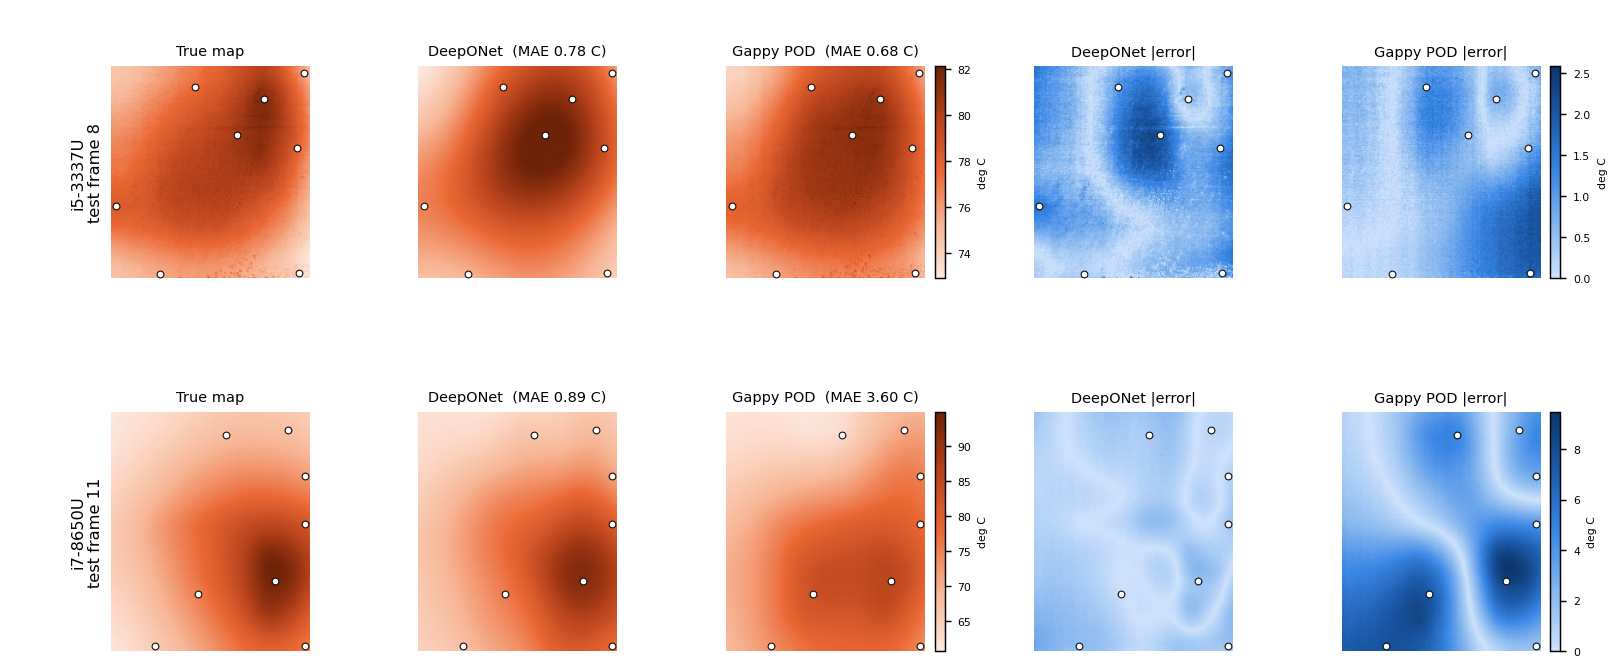
\includegraphics[width=\textwidth]{figures/real_maps_n8_crop.png}
\caption{Measured IR maps with 8 sensors (white dots), one typical test frame per processor (seed 0). From left: measured map, DeepONet, gappy POD (sharing one temperature scale), and the absolute errors of DeepONet and gappy POD.}
\label{fig:real_maps}
\end{figure*}

\subsection{Pure PINN on measured maps}
Because each PINN solve takes minutes, the per-frame PINN was run on a regular sample of frames: 10 validation and 10 test frames for the i5 and 20 and 20 for the i7.
Table~\ref{tab:real_frames} compares all models on exactly these frames and readings; its DeepONet and hybrid values differ slightly from Table~\ref{tab:real}, which uses every test frame.
With all training workloads the PINN is much weaker than the DeepONet (for example 0.70 against 0.23 at 5 sensors on the i7), and blending it in does not help; on the i5 it hurts, because the single validation workload is unlike the test workload and the blend over-trusts the PINN.
The correction hybrid is better than the DeepONet at i5/8 and i7/10 sensors, tied in the other four settings, and better than the PINN in all six.

\begin{table}[t]
\caption{Measured IR maps, sampled test frames (i5: 10, i7: 20), all training workloads. Error relative to the temperature rise. DeepONet, blend and hybrid: mean of 5 seeds; PINN: 1 seed per frame.}
\label{tab:real_frames}
\centering
\footnotesize
\setlength{\tabcolsep}{2.4pt}
\begin{tabular}{@{}l ccc ccc@{}}
\toprule
& \multicolumn{3}{c}{i5-3337U} & \multicolumn{3}{c}{i7-8650U} \\
\cmidrule(lr){2-4}\cmidrule(l){5-7}
Model & $N{=}5$ & 8 & 10 & 5 & 8 & 10 \\
\midrule
DeepONet & .209 & .150 & .149 & \best{.230} & .110 & .107 \\
Per-frame PINN & .762 & .233 & .236 & .695 & .371 & .176 \\
Blend (DeepONet + PINN) & .416 & .182 & .201 & \best{.230} & .110 & .097 \\
Hybrid (correction) & .229 & .132 & .139 & \best{.229} & \best{.106} & .091 \\
Gappy POD & \best{.124} & \best{.100} & \best{.137} & .370 & .221 & \best{.085} \\
Training-mean map & .956 & .956 & .956 & .905 & .905 & .905 \\
\bottomrule
\end{tabular}
\end{table}

\subsection{Physics helps when training workloads are scarce}
To test the central claim on measured data, the i7 DeepONet was retrained on only 1, 2 or 4 of its 13 training workloads (nested, seeded subsets; the sensor layout fitted on all 13 is kept); the PINN and the physics correction use no training maps and are unchanged.
Fig.~\ref{fig:real_lowdata} and Table~\ref{tab:real_low} show the result, which mirrors Fig.~\ref{fig:lowdata}.
The DeepONet degrades sharply, from 0.11 to 0.43 at 8 sensors with 2 workloads, and with the single idle workload it fails completely (error about 2.5).
The hybrid holds up: with 4 workloads it lowers the DeepONet's error from 0.356 to 0.163 at 8 sensors and from 0.338 to 0.143 at 10 sensors, reductions of more than half, and at 8 sensors it also beats the PINN (0.371) by a similar margin.
Paired over test frames, the hybrid is better than the DeepONet at 8 and 10 sensors with both 2 and 4 workloads and at 5 sensors with 2 workloads, and ties at 5 sensors with 4 workloads.
With all 13 workloads the same hybrid gains only 0.001--0.016.
At 10 sensors with 2 workloads the PINN alone is about as good (0.176 vs 0.191, a tie), consistent with the bias--variance view: when the learned model is very weak, the best estimate is close to the physics one.

\begin{figure*}[t]
\centering
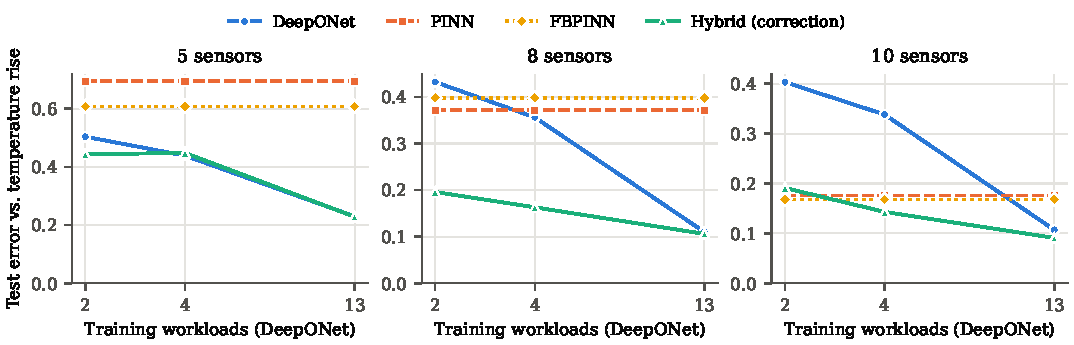
\includegraphics[width=\textwidth]{figures/real_low_data.pdf}
\caption{Measured IR maps (i7, 20 sampled test frames): test error relative to the temperature rise against the number of training workloads given to the DeepONet. The per-frame PINN uses no training maps. The hybrid (DeepONet + physics correction, 5 seeds) stays far below the DeepONet when workloads are few and converges to it when all are available.}
\label{fig:real_lowdata}
\end{figure*}

\begin{table}[t]
\caption{Measured IR maps, i7, 20 sampled test frames: error relative to the temperature rise when the DeepONet is trained on 2, 4 or all 13 workloads. DeepONet, blend and hybrid: mean of 5 seeds; PINN: 1 seed, no training maps.}
\label{tab:real_low}
\centering
\footnotesize
\setlength{\tabcolsep}{3pt}
\begin{tabular}{@{}cc cccc@{}}
\toprule
$N$ & Workloads & DeepONet & PINN & Blend & Hybrid (correction) \\
\midrule
\multirow{3}{*}{5}  & 2  & .504 & .695 & .495 & \best{.444} \\
                    & 4  & \best{.439} & .695 & \best{.439} & .448 \\
                    & 13 & .230 & .695 & .230 & \best{.229} \\
\midrule
\multirow{3}{*}{8}  & 2  & .432 & .371 & .270 & \best{.196} \\
                    & 4  & .356 & .371 & .293 & \best{.163} \\
                    & 13 & .110 & .371 & .110 & \best{.106} \\
\midrule
\multirow{3}{*}{10} & 2  & .403 & \best{.176} & .179 & .191 \\
                    & 4  & .338 & .176 & .203 & \best{.143} \\
                    & 13 & .107 & .176 & .097 & \best{.091} \\
\bottomrule
\end{tabular}
\end{table}

%=====================================================================
\section{Discussion}\label{sec:discussion}

\subsection{When and how physics helps}
Across both datasets the answer is consistent.
Physics added as a \emph{loss term} to a network trained on hundreds of supervised maps is neutral at best.
Physics used as a \emph{separate, data-free estimator} combined with the learned operator helps, and its benefit is governed by the amount of training data: with plentiful data it adds at most 0.4 points on simulated dies and 0.001--0.016 in rise error on measured maps, but with 25 training chips it removes a third of the DeepONet's error and with 2--4 training workloads more than half.
The selected blend weights follow the trade-off of Section~\ref{sec:biasvar}, moving towards the physics estimator as training data shrink.
A second, data-independent benefit is that the physics estimator recovers the peak temperature that the learned model flattens.

\subsection{Why physics as a loss adds little}
Passing the simulated reference maps themselves through a $128\times128$ finite-volume discretisation of (\ref{eq:pde}) leaves a pointwise residual of 32.9\% of the signal (40 validation chips).
99\% of its squared magnitude sits in the worst 5\% of pixels, at hot spots and sharp block edges; it falls to 7.0\% away from block edges and to 7.9\% when averaged over $16\times16$ patches.
The references come from a finer mesh with sharp, block-wise sources that a coarse grid operator cannot reproduce exactly, which is the price of avoiding an inverse crime and a fair picture of real chips, whose physics is never known exactly.
A PDE loss on the coarse grid therefore asks the network to move away from the very maps it is fitted to, exactly where errors are largest.
The blend and the correction avoid this conflict: the physics model makes its own prediction, and validation data decide how much of it to keep.

\subsection{Implications for thermal measurement}
(i) A trained DeepONet produces a full map in tens of milliseconds, fast enough for run-time monitoring; a per-chip PINN takes minutes and suits design-time analysis or a slower supervisory loop.
(ii) Learned models systematically under-estimate the peak temperature; a physics-based estimate or correction should inform any throttling decision.
(iii) For a new product or measurement campaign with few recorded maps, a hybrid is the safer choice than a purely data-driven model.
(iv) On smooth real maps with 10 sensors, gappy POD can match a network, so a classical baseline must always be reported.

\subsection{Limitations}
The simulated dies use a two-dimensional compact model with uniform power per block and constants ($t_\mathrm{die}$, $h_\mathrm{eff}$, power ranges) that are plausible but not traced to a specific product.
Sensor positions come from POD-QR only; we did not compare alternative placements.
Several entries rest on one seed (the PINN, the blend); we report the seed count for every entry and paired confidence intervals for the main claims.
The real-data study covers two processors; the i5 has a single validation and a single test workload, the IR maps are smooth and camera-blurred, and the rule for choosing the real-data hybrid variant was fixed after some per-seed test numbers had been seen.
The per-frame PINN was run on sampled frames with a shortened budget; frames within a workload are strongly correlated, so frame-level confidence intervals are optimistic, and the scarcity study on real maps covers the i7 only.
Only steady state is modelled.

%=====================================================================
\section{Other Architectures Explored}\label{sec:other}

Before settling on the DeepONet we trained four other physics-informed architectures on the simulated set under the same protocol (Table~\ref{tab:other}).
All learn across chips from an encoding of the sensor readings and predict both temperature and source, with a physics residual weighted 0.01 unless stated.
These runs had smaller budgets and mostly one seed, so the table is a survey, not a ranking.

\begin{table}[t]
\caption{Other architectures on the simulated test set (500 training chips unless stated). Relative $L_2$ error (\%). Seeds listed per sensor count; multi-seed entries are mean $\pm$ s.d.}
\label{tab:other}
\centering
\footnotesize
\setlength{\tabcolsep}{3pt}
\begin{tabular}{@{}l c ccc@{}}
\toprule
Model & Seeds & $N{=}5$ & $N{=}8$ & $N{=}10$ \\
\midrule
DeepONet (reference) & 5/5/5 & 11.46 & 8.62 & 6.13 \\
FNO/PINO & 1/1/3 & 13.20 & 10.79 & 9.78{\scriptsize$\pm$.20} \\
FBPINN, physics on & 1/3/3 & 11.35 & 8.95{\scriptsize$\pm$.05} & 6.76{\scriptsize$\pm$.03} \\
FBPINN, physics off & --/--/1 & -- & -- & 6.83 \\
XPINN, physics on$^\ast$ & 1/1/3 & 11.43 & 8.72 & 6.45{\scriptsize$\pm$.03} \\
XPINN, physics off & 1/1/1 & 11.38 & 8.63 & 6.40 \\
Solver hybrid / data-only twin & --/--/1 & -- & -- & 6.58 / 6.53 \\
\quad 50 training chips & --/--/1 & -- & -- & 10.81 / 9.79 \\
\quad 25 training chips & --/--/1 & -- & -- & 12.58 / 11.48 \\
\bottomrule
\multicolumn{5}{@{}p{0.95\columnwidth}}{\footnotesize $^\ast$Physics residual masked next to tile edges; without the mask: 16.2\% at $N{=}10$.}
\end{tabular}
\end{table}

\emph{FNO/PINO} \cite{li2021fno,li2024pino}: a Fourier neural operator (4 spectral layers, 8 modes, $5.3\times10^5$ parameters) with a physics loss.
It needs gridded input, so the sparse readings must be scattered onto an almost empty grid, which suits spectral layers poorly.
It had the highest error of all models, became worse with a larger physics weight (13.6 vs 10.4\% at 3000 steps with weight 0.1), and on the IR maps one training step took 2.8\,s on our CPU, so a budget equal to the DeepONet's was not feasible.

\emph{FBPINN} \cite{moseley2023fbpinn}: 9 overlapping windows, each with a small network, blended by smooth weights.
It came within 0.6 points of the DeepONet with a fifth of its parameters, but switching the physics off changed nothing (6.76 vs 6.83\%).
As a per-frame solver on the IR maps (2$\times$2 windows, the same frames and budget as the PINN) it beat the PINN in 4 of 6 settings and tied in 2, but cost about three times as much per frame and remained worse than the DeepONet in all six; blending it with the DeepONet did not change the validation choice of hybrid.

\emph{XPINN} \cite{jagtap2020xpinn}: $3\times3$ non-overlapping tiles coupled by interface losses.
With physics on it stalled at 16\% error, because output jumps at tile edges create large residuals that the optimiser removed by flattening the field; masking the residual next to tile edges fixed this (6.45\%), but the result then matched the physics-off model (6.40\%), and the maps showed visible seams.

\emph{Solver hybrid}: a network predicts the heat source and a differentiable grid solver of (\ref{eq:pde}) computes the temperature, so every prediction satisfies the discretised physics.
It tied its data-only twin with 500 chips and was about 1 point \emph{worse} with 25 or 50 chips: forcing the prediction through a physics that the references do not satisfy exactly removes exactly the flexibility that scarce data cannot replace.
A data-driven PINN trained across all chips gave a similarly small effect in a short preliminary run (6.23 vs 6.45\% with and without physics, one seed).

Together these results support the choice of the DeepONet: none of the alternatives was more accurate; each carried a practical cost (gridded input and slow training for the FNO, tile seams for the XPINN, three times the per-frame cost of the PINN for the FBPINN, a full grid solve for the solver hybrid); and in none did physics in the loss help, which is what led us to study physics as a separate estimator.

%=====================================================================
\section{Conclusion and Future Work}\label{sec:conclusion}
We studied full-chip thermal map reconstruction from 5 to 10 noisy sensors as an operator-learning problem and asked when the heat equation helps a DeepONet.
With 500 training chips the DeepONet reconstructs simulated maps to 6--11\% relative error in milliseconds, and physics as a loss term gives no measurable gain.
Physics as a separate estimator, combined with the DeepONet through validation-chosen weights, is never worse than its better component and becomes more valuable as training data shrink, cutting the error by a third with 25 training chips; on measured IR maps of an Intel i7 a physics correction more than halves the DeepONet's error at 8 and 10 sensors when only 2 or 4 training workloads are available.
The blend weights follow a bias--variance trade-off between a low-bias learned operator and a data-free physics estimator, and the physics estimator also recovers peak temperatures that the learned model flattens.
Future work includes transient reconstruction, learning sensor placement jointly with the reconstruction, uncertainty estimates for the combined map, three-dimensional die-and-package models, and validation on more processors with measured power.

\section*{Data and Code Availability}
\todo{Repository URL and licence. The real IR maps are not redistributed; they are available from the original authors \cite{lu2024dataset}.}

\section*{Acknowledgment}
\todo{Funding and acknowledgements.}

\bibliographystyle{IEEEtran}
\bibliography{refs}

\end{document}
